\section{实验：结构优势何时转化为查询收益}\label{sec:evaluation}
实验研究四个问题：固定协议参数时，历史增长是否保持小的可达接口状态；容量增加何时使编译不再可行；新假设数量和局部分解如何改变收益；完整支持在按需诊断中能否抵消构造费用。所有数据来自冻结实现和结果，本文绘图只重新整理已有测量。

\subsection{比较方法与测量范围}
比较四种方法。B0 直接从原始事件和值／守卫构建 RA SAT 编码，不使用协议证书；B1 使用同一证书简化后的增量 SAT；BD 在 B1 公式上做单位传播，以残余 CNF 的变量关联图提取静态组件并使用局部缓存；B2 是本文的二元 RF、稀疏直接 CO 和联合端口编译。BD 的分区包含辅助变量，也检查纯辅助组件，不读取阶段编号或预设每轮模型数。B0/B1 复用 CaDiCaL 的学习信息，用模型批量发现支持，再询问尚未发现支持的析取，避免逐文字重启。

完整支持接口比较中，四者使用相同的完整答案缓存，命中后仍形成全部原始文字的排序输出。主缓冲扫描每个输入有 $Q=1000$ 次请求，通常全部为不同假设；$C=2$ 的请求池有 $997$ 个不同假设和 $3$ 次命中。其中 $990$ 个可满足条件长度为 $4$，且逐文字不可冗余；其余为长度 $2$ 的删除极小冲突。条件来自仍未固定的 RF／CO 位，排列文字或添加常量不产生新请求。请求池在计时外固定，各方法接收相同条件。第~\ref{sec:diagnosis}节的任务比较则按实际需要区分一致性、字段支持和完整快照。

主测量在 Windows 11、Python 3.12.14、python-sat 1.8.dev30 和 CaDiCaL195 下进行，每个性能进程使用一个 CPU；B2 使用 Python 端口更新。成功主点和诊断点均有三次独立进程重复，图中点或柱为中位数，误差线为最小值至最大值。超时／预算失败点各保留一次。进程墙钟预算为 $60$ 秒，B2 另有 $200\,000$ 状态、$600\,000$ 转移和 $50$ 秒编译预算。报告的算法时间包含证书、构造、查询及实际输出，审计哈希和文件写入不计入；进程预算还涵盖这些外围开销。内存采用工作进程自身的操作系统峰值，超时点以整棵进程树另行复核。

缓冲采用第~\ref{sec:buffer}节的分支观测，槽负载值固定，保留跨阶段多来源；其单写者索引和槽访问使全部 CO 固定。屏障采用第~\ref{sec:barrier}节的两个工作者和一个协调者，数据区为所示六事件访问，$p=3,a=6,B=3$，保留多写者 RF／CO 耦合。这两个族分别检验不同结构，不能合并声称每个输入都同时具有全部特性。查询复用和布局消融来自独立冻结批次，以下单独标明。

\subsection{固定容量下的历史增长}\label{sec:historyexp}
图~\ref{fig:historycost} 固定 $C=3$，把成功操作对的轮数 $r$ 从 $4$ 增至 $32$。B2 的冷启动加千次完整支持成本由 \HistoryFour\ 秒增至 \HistoryThirtyTwo\ 秒。在 $r=8$ 时，B2 为 \BufferEightBTwo\ 秒，BD 为 \BufferEightBD\ 秒；后者已经具有相同证书和组件缓存。$r=16,32$ 时三个 SAT 方法均未在进程预算内完成整个请求序列，因此图中保留超时标记，不从 $60$ 秒计算精确加速比。

\begin{figure}[t]
\centering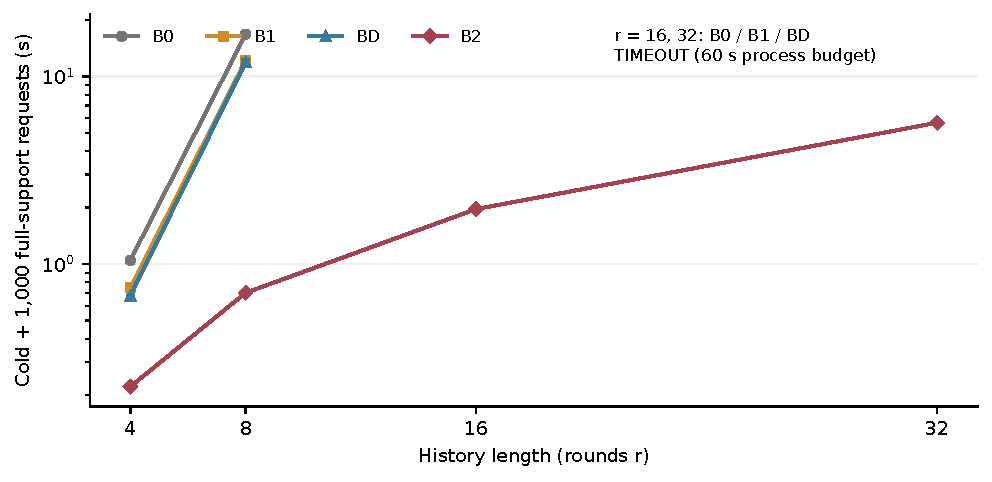
\includegraphics[width=.96\linewidth]{figures/history_cost.pdf}
\caption{分支缓冲固定 $C=3$ 的历史增长。横轴为轮数 $r$，纵轴为冷启动加 $1000$ 次完整支持请求的秒数，对数刻度；成功点为三次重复的中位数及最小／最大范围。未完成点不作为成功曲线点。主缓冲扫描批次。}\label{fig:historycost}
\end{figure}

图~\ref{fig:historystates} 和表~\ref{tab:historystructure} 将关系压缩与输出规模分开。最大层状态 $S_{\max}$ 始终为 $30$，总状态和转移随历史有规律地增长；每轮仍增加真正有多个来源的读。与此同时，原始变量数从 $108$ 增至 $5680$。这些变量含退休事件及常量，完整支持服务必须继续回答它们。$32$ 轮的查询部分约为 $4.82$ 秒，超过约 $0.53$ 秒的图编译时间。恒定 $S_{\max}$ 因此不意味着恒定端到端时间或内存。成功工作进程的最大峰值约为 $691$ MiB，全部低于 $1$ GiB；六个超时点的进程树复核仍为时间超限，峰值为 $111$--$221$ MiB。

\begin{figure}[t]
\centering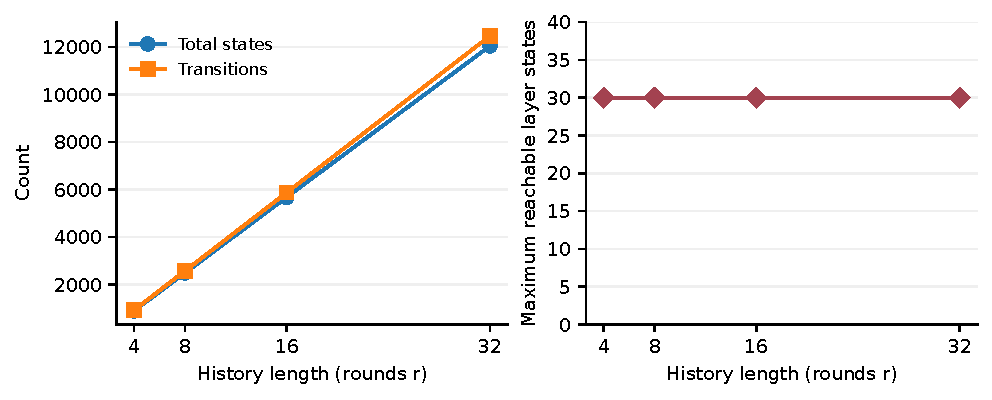
\includegraphics[width=.96\linewidth]{figures/history_states.pdf}
\caption{同一 $C=3$ 扫描的状态规模。左图为总状态／转移，右图为最大可达层状态；两者均为计数，各自使用独立纵轴。三次成功重复的结构统计一致。理论中的指数上界 $S_{\rm bd}$ 不在本图中充当预测值。}\label{fig:historystates}
\end{figure}
\begin{table}[t]
\centering\small
\caption{固定 $C=3$ 的缓冲结构。$n$ 包含初始化事件；$|D|$ 为剩余 RF 候选总数；所有输入的未决 CO 数均为零。}\label{tab:historystructure}
% Generated from frozen JSON; do not edit.
\begin{tabular}{rrrrrrrrrr}
\toprule
$r$ & $n$ & $|X|$ & $|D|$ & 歧义读 & $K$ & 组数 & $S_{\max}$ & 状态 & 转移 \\
\midrule
4 & 38 & 108 & 30 & 6 & 10 & 122 & 30 & 899 & 928 \\
8 & 70 & 388 & 66 & 14 & 12 & 234 & 30 & 2491 & 2576 \\
16 & 134 & 1464 & 138 & 30 & 12 & 458 & 30 & 5675 & 5872 \\
32 & 262 & 5680 & 282 & 62 & 12 & 906 & 30 & 12043 & 12464 \\
\bottomrule
\end{tabular}

\end{table}

这种压缩也不依赖把缓冲各阶段拆成互不关联的小问题。预处理后的 CNF 在每个主缓冲输入中都有一个包含全部未固定原始位的组件。连通性本身只描述公式表示；额外的原始语义核查给出真正跨阶段关联：在 $16$ 轮、$C=3$ 输入中，$\RF{W_8}{Q5\_peer}$ 与 $\RF{A_6}{P6\_peer}$ 分别可满足，但合取不可满足。它们分属第 $6$ 和第 $7$ 阶段，排除了这两个阶段选择完全独立的解释。$8$ 轮、$C=4$ 还具有第 $6$ 与第 $8$ 阶段的相应冲突。

\subsection{容量扩大与可达状态预算}\label{sec:capacityexp}
表~\ref{tab:capacity} 固定 $r=8$ 改变容量。$C$ 从 $3$ 到 $4$ 时，$K$ 从 $12$ 增至 $15$，而 $S_{\max}$ 从 $30$ 增至 $294$，状态总数增长明显快于处理组数。B2 仍可完成，但构造和千次支持查询的总时间增至约 $4.21$ 秒。这说明容量窗口会实质影响联合状态，不只增加若干事件。

\begin{table}[t]
\centering\small
\begin{threeparttable}
\caption{固定 $r=8$ 的容量扫描。时间为冷启动加 $1000$ 次完整支持请求的秒数，成功点取三次中位数。}\label{tab:capacity}
% Generated from frozen JSON; do not edit.
\begin{tabular}{rrrrrrrr}
\toprule
$C$ & $\max|D(r)|$ & $K$ & 组数 & $S_{\max}$ & 状态 & BD (s) & B2 (s) \\
\midrule
2 & 2 & 9 & 219 & 4 & 501 & 3.6265 & 0.2857 \\
3 & 3 & 12 & 234 & 30 & 2491 & 11.8927 & 0.7028 \\
4 & 4 & 15 & 247 & 294 & 16819 & 22.8425 & 4.2130 \\
6 & 6 & 17 & 267 & $\ge 12420$\tnote{a} & 200001\tnote{a} & 38.2462 & 状态上限 \\
\bottomrule
\end{tabular}

\begin{tablenotes}[flushleft]\footnotesize
\item[a] $C=6$ 在第 $187$ 个处理步骤触发状态预算；所列状态是失败时的部分计数，$S_{\max}$ 仅为完整构造的下界。\texttt{STATE\_LIMIT} 表示没有进入查询。
\end{tablenotes}
\end{threeparttable}
\end{table}

$C=6$ 在约 $28.38$ 秒触及状态预算，此时已产生 $200\,001$ 个状态和 $205\,322$ 条转移。B0、B1、BD 则均完成，分别约为 $47.41$、$37.49$ 和 $38.25$ 秒。因此当前实现的正面区间是已测的 $C=2,3,4$；$C=6$ 给出明确的工程边界。没有测量的 $C=5$ 不能被当作已经定位的阈值，状态预算失败也不意味着扩大预算后一定无法构造。容量、候选域、$K$ 和可达状态同时变化，测量支持整体机制解释，不把全部耗时差异归给单一结构参数。

为检查对请求池的敏感性，另在 $r=8,C=3$、$r=4,C=3$ 和 $r=8,C=4$ 各使用两个新池，每池测试原顺序和固定洗牌，每个设置两次重复。四组池／顺序的 B2/BD 总时间比分别处于 $0.055$--$0.064$、$0.284$--$0.321$、$0.178$--$0.185$，优势方向未改变。这只覆盖既定的假设长度及 SAT 比例分布。$r=4,C=3$ 是成功点中比值最接近 $1$ 的点，但仍明显有利于 B2，不是一个实测收益交叉点。

\subsection{新假设、局部复用和布局的解释}\label{sec:reuseexp}
图~\ref{fig:reuse} 使用独立的屏障查询复用批次，固定 $Q=1000$，令不同全局假设数 $U$ 为 $21,100,500,1000$。$U=21$ 时共有 $979$ 次全局答案命中；$U=1000$ 时全部请求都是新条件。随着全局复用降低，B1 成本显著增加，B2 的图扫描成本也增加。BD 却能继续复用局部结果，并在全部新条件时优于 B2。

\begin{figure}[t]
\centering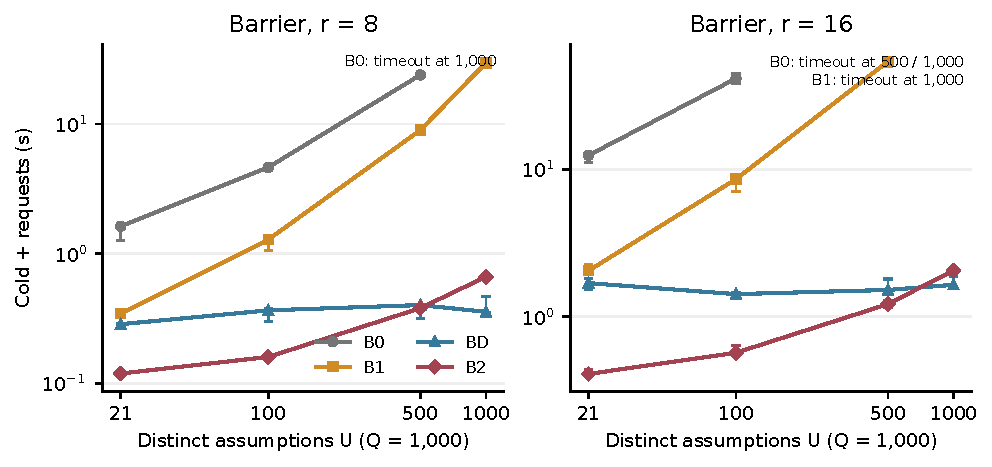
\includegraphics[width=.96\linewidth]{figures/query_reuse.pdf}
\caption{屏障上全局新假设数量与成本。$Q=1000$，横轴为不同假设数 $U$；纵轴为冷启动加请求成本，秒，对数刻度。成功点三次重复，中位数及最小／最大范围；标注的超时点没有绘制虚构耗时。该图来自查询复用批次，独立于图~\ref{fig:historycost} 的主缓冲扫描。}\label{fig:reuse}
\end{figure}

原因可以直接核查。在可穷举的 $1,2,3$ 轮上，完整关系分别有 $9,81,729$ 个模型，并等于按工作区分解后的直积，跨轮原始位固定。在实际 $8,16$ 轮残余 CNF 中，自动组件提取分别得到 $8,16$ 个含原始自由位的组件，每个有 $6$ 个原始自由位和 $9$ 个局部模型。BD 不需要知道轮号便可以利用这一结构。当 $U=1000$ 时，$8,16$ 轮 BD 只有 $82,154$ 次局部缓存缺失，尽管全局缺失各为 $1000$。表~\ref{tab:reuse} 给出这些请求及答案数量。所测屏障的恒定层状态并不能证明持续的跨轮关联；缓冲的语义反例承担了后一项证据。

\begin{table}[t]
\centering\small
\caption{屏障查询复用的解释量。不同完整答案数包含统一的不可满足答案；时间为三次中位数。局部缺失统计来自 BD 自动提取的 CNF 组件。}\label{tab:reuse}
% Generated from frozen JSON; do not edit.
\begin{tabular}{rrrrrrrr}
\toprule
$r$ & $U$ & 全局命中 & 不同答案 & BD 局部缺失 & B1 (s) & BD (s) & B2 (s) \\
\midrule
8 & 21 & 979 & 12 & 51 & 0.3451 & 0.2854 & 0.1188 \\
8 & 100 & 900 & 91 & 82 & 1.2814 & 0.3647 & 0.1594 \\
8 & 500 & 500 & 491 & 82 & 8.9654 & 0.4008 & 0.3793 \\
8 & 1000 & 0 & 991 & 82 & 29.6376 & 0.3552 & 0.6621 \\
16 & 21 & 979 & 12 & 66 & 2.0491 & 1.6897 & 0.4088 \\
16 & 100 & 900 & 91 & 150 & 8.5698 & 1.4225 & 0.5693 \\
16 & 500 & 500 & 491 & 154 & 53.9582 & 1.5183 & 1.2179 \\
16 & 1000 & 0 & 991 & 154 & 超时 & 1.6464 & 2.0603 \\
\bottomrule
\end{tabular}

\end{table}

布局消融也显示宽度界与实测成本的区别。$16$ 轮屏障的稀疏 CO 表示为 $K=13$，冷启动加 $100$ 次查询约 $0.516$ 秒；稠密 CO 为 $K=162$，约 $2.878$ 秒。但稠密化还增加了处理组和状态数，不能把约 $5.6$ 倍差异全部解释为 $K$ 的单独作用。普通输入布局取 $K=15$，约 $0.493$ 秒，反而略快于专用布局。长写间隔变体中，专用／普通布局在 $16$ 轮分别为 $K=15/17$、约 $0.525/0.489$ 秒。附录表~\ref{tab:mechanism} 同时列出组、状态、转移及计划、编译、查询分项。理论贡献是一个有证明且无需搜索的构造，实际耗时还由可达状态、处理组数和计划费用决定。

\subsection{按需诊断中的收益反转}\label{sec:diagnosis}
我们把第~\ref{sec:queries}节的日志编辑任务应用于 $8$ 轮屏障与 $8$ 轮、$C=3$ 缓冲。每份输入含 $32$ 段日志，其中 $16$ 段具有跨字段冲突，$16$ 段为对应一致记录。客户端加入字段、求删除极小冲突、枚举全部单字段修复、选择确定排序的首个修复，再撤销和恢复一个字段。四种方法得到相同冲突、修复集合与支持快照；屏障共有 $32$ 个替代修复，缓冲共有 $46$ 个。

两种输出模式改变任务需求。最终快照模式只在每段末尾输出一次完整支持，共 $32$ 次；频繁快照模式还在一致编辑后输出，共 $128$ 次。两者均另有 $208$ 次一致性请求和 $32$ 次字段支持请求。B0/B1 的删除检查只问 SAT，修复只求目标字段；BD 限定到相关组件，B2 用可达性做一致性。相同的是请求及其结果，不要求相同内部 SAT 调用次数。

\begin{figure}[t]
\centering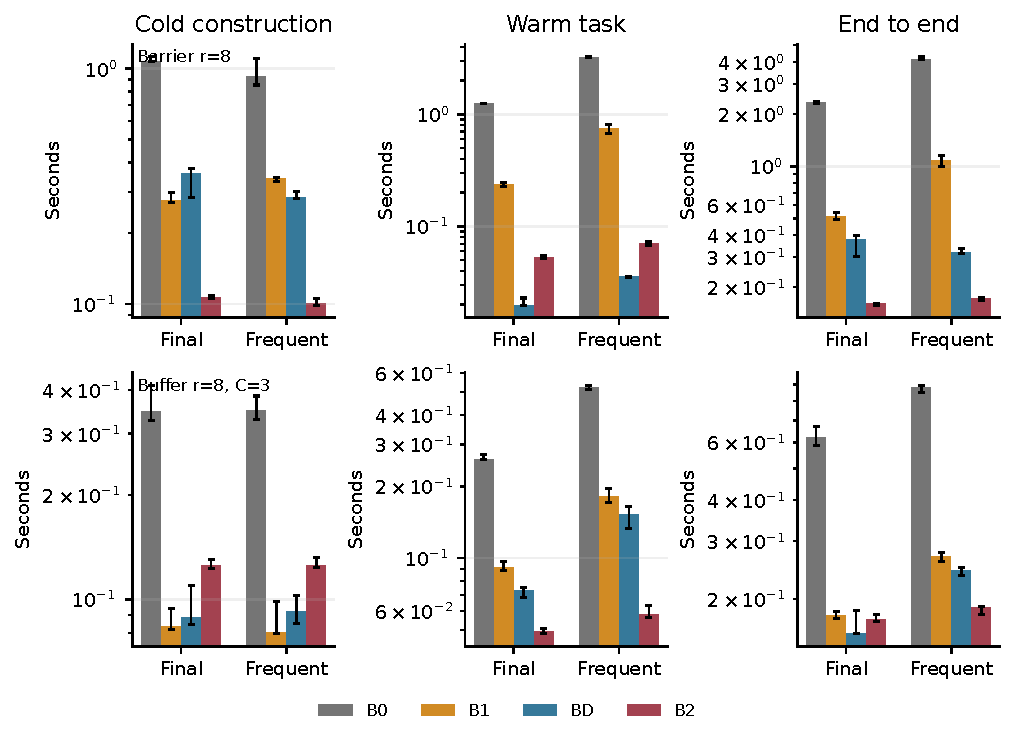
\includegraphics[width=\linewidth]{figures/diagnosis.pdf}
\caption{相同日志诊断任务的冷启动、温态与端到端成本，单位秒，均为对数刻度。Final 为最终快照，Frequent 为频繁快照；每点三次进程重复，柱为中位数，误差线为最小／最大范围。三个分项独立统计并分图绘制，没有把独立中位数强行堆叠。诊断批次包含结果序列化费用。}\label{fig:diagnosis}
\end{figure}

图~\ref{fig:diagnosis} 显示任务结构可以改变方法排名。缓冲最终快照模式中，BD 为 \BufferSparseBD\ 秒，B2 为 \BufferSparseBTwo\ 秒；温态查询收益不足以覆盖 B2 更高的冷启动成本。频繁快照模式中，BD 为 \BufferDenseBD\ 秒，B2 为 \BufferDenseBTwo\ 秒，B2 才取得端到端优势。其幅度约为 $1.30$ 倍，显著小于主接口实验千次新完整支持请求的约 \BufferRatio\ 倍。两种请求结构不能互换加速比。

屏障又体现另一种成本来源。BD 的最终／频繁快照温态约为 $0.0198/0.0354$ 秒，快于 B2 的 $0.0524/0.0700$ 秒；B2 的端到端领先伴随更低构造成本。结果支持按任务需求选择复用方式：同一套精确支持表示可以服务多种请求，但完整编译的投入是否值得，要连同冷启动、局部缓存及完整快照频率一起判断。

\subsection{正确性证据与适用边界}
小实例检查直接比较完整原始赋值集合：对 $36$ 个可枚举案例分别枚举 RF 与逐地址 CO，与接受路径投影双向核对；另对极小输入穷举 $1152$ 个布尔原始赋值，包含违反恰一 RF 或总 CO 的非法赋值。查询核对覆盖条件冲突、撤销、已退休事件和固定原始位。单轮屏障工作区的 $9$ 个模型中有 $2$ 个 RF／CO 赋值没有 SC 线性化，这没有把整个读值观测误称为 SC 不可达。

较大输入采用不读取 $D/H/L$ 的原始 RA SAT 编码，核查 $494$ 个预先选定的排除：$168$ 个永久删除 RF、$168$ 个固定 CO 的反向、$158$ 个条件下不支持文字，全部不可满足，无未知结果。条件样本中 $134$ 个来自缓冲跨阶段关联，$24$ 个来自屏障局部关联。对条件本身和撤销条件后恢复的目标文字做正对照，加上根输入共 $323$ 次可满足检查；所获完整赋值再按独立的稠密 $\hb/\eco$ 定义验证。样本覆盖容量边界、模数回绕、失败尝试、失败尾链和未完成调用。这里独立的是原始语义编码相对于协议过滤及编译图；没有第二套 SAT 求解器或 DRAT/LRAT 证明日志。$32$ 轮输入只在已完成基线的公共请求前缀上比较完整答案，不能把 B2 的全部千次结果称为已获原始 SAT 全量确认。

这些实例是来自明确协议结构的生成观测，尚无工业日志覆盖率调查。更早的重复发布内核还保留了恒定载荷六轮构造超预算、四轮按需 SAT 更快的结果；改用轮次版本值会缩小来源域，这部分收益来自观测信息增加。第一轮屏障测量中，温态 SAT 和单文字查询也快于完整支持扫描。这些结果共同限定性能主张：协议界说明存在可控的候选接口，具体收益仍取决于可达状态、可提取分解、输出规模和请求类型。BD 只是静态组件基线；没有同投影任务上的成熟编译器对照，实验不支持胜过通用知识编译工具的结论。
